\documentclass[11pt,a4paper]{article}

\usepackage[margin=0.85in]{geometry}
\usepackage{amsmath,amssymb,amsthm}
\usepackage{booktabs}
\usepackage{graphicx}
\usepackage{xcolor}
\usepackage{enumitem}
\usepackage{hyperref}
\usepackage{fancyhdr}
\usepackage{float}

\hypersetup{
  colorlinks=true,
  linkcolor=blue!60!black,
  citecolor=blue!60!black,
  urlcolor=blue!60!black
}

\newtheorem{proposition}{Proposition}
\newtheorem{definition}{Definition}

% Macro for unrun solver results so no unverified metric is ever fabricated
\newcommand{\pending}[1]{\textcolor{orange!75!black}{\texttt{[PENDING: #1]}}}

\pagestyle{fancy}
\fancyhf{}
\lhead{Ladle Turnover and Single-Track Crane Scheduling}
\rhead{Page \thepage}
\renewcommand{\headrulewidth}{0.4pt}

\begin{document}

% ============================================================================
% ONE-PAGE EXECUTIVE SUMMARY SHEET
% ============================================================================
\thispagestyle{empty}
\begin{center}
  {\LARGE \textbf{Safe Spatio-Temporal Coordination of Multi-Crane Ladle Handling in Steelmaking--Refining--Continuous Casting}}\\[0.4em]
  {\large \textit{Executive Summary Sheet}}
\end{center}
\vspace{0.2em}
\hrule
\vspace{0.6em}

\noindent\textbf{Industrial Context \& Forensic Diagnosis.}
In integrated steelmaking--refining--continuous casting (SCC) plants, molten steel is transported across converters (BOF), secondary refining stations (LF, RH), and continuous casters (CCM) by overhead cranes sharing a single runway. Analysis of 12 production workbooks (17.5 days; 6,758 raw rows; 1,321 tapping plans including 55 \texttt{-2} placeholders and 1,266 operational heats across 152 casts) reveals that \emph{inter-stage queueing rather than crane transit} dominates cycle time: nominal plans embed fixed 15--30~min inter-stage buffers, whereas median observed tapping, LF, RH, and casting durations are 5.63, 36.92, 39.00, and 40.65~min, respectively, and inter-heat caster gaps in cast \texttt{6C0754} compress to 1.53--2.78~min. Non-destructive auditing further uncovers 2,529 candidate anomalies---including 72 duplicate heat IDs in the summary log, 533 zero-span RH degassing timestamps, 323 missing lift records in \texttt{3\#LF}, and empty-ladle return weights reaching 137.0--149.9~t (explaining why 150~t auxiliary cranes are bypassed in favor of 450~t cranes on the E--F bay).

\noindent\textbf{Unified Framework \& Scenario 1 (Deterministic Baseline).}
We establish a unified heat-event network coupled with single-track non-crossing crane scheduling along the verified west-to-east E--F crane sequence $\text{2\#150} \prec \text{4\#450} \prec \text{3\#450} \prec \text{5\#450} \prec \text{1\#150}$. The task set captures four coupled move classes: forward heavy-ladle transfers (405.5--421.3~t), post-casting empty returns (direct, slag-dumping, or residue-recovery branches to transfer cars \texttt{1\#--3\#}), converter-C empty-ladle supply, and dual-heat cast-residue recovery. Under a lexicographic objective---(1) collision-free safety and cast continuity, (2) minimum heat waiting, and (3) minimum crane travel---we prove that enforcing separation at trajectory breakpoints is necessary and sufficient for continuous-time safety under constant speeds. On historical replay of cast \texttt{6C0754} (6 heats, 18 primary moves), \texttt{3\#450} absorbs 116.87~min of crane duty versus 72.40~min on \texttt{5\#450} and 14.35~min on \texttt{4\#450}, while cast-start delay drifts from $-0.93$~min to $+19.00$~min and thermal age escalates from 9.98 to 31.72~min. \pending{Insert full-day EDF vs. rolling CP-SAT wait/runtime reductions and 150~t offload boundary.}

\noindent\textbf{Scenario 2 (Multi-Gear Kinematics \& Stochastic Processing).}
To address stochastic processing times, acceleration/braking, discrete crane gears, and spatial slow-down zones, we formulate a forward--backward $v^2(x)$ velocity-envelope trajectory builder paired with chronological day-block bootstrapping and a non-anticipative rolling Sample Average Approximation with Conditional Value-at-Risk ($\text{SAA-CVaR}_\alpha$) on critical cast-readiness tardiness. \pending{Insert out-of-sample P95 wait, cast-break rate, and paired policy cost difference.}

\noindent\textbf{Scenario 3 (Fault-Resilient Rescheduling).}
We distinguish micro-perturbations (tapping delays, argon-station/ladle-car occupancy) from four macro-faults (BOF, refining, CCM, and crane breakdowns). We prove a topological rail-partitioning condition: a disabled mid-bay crane physically splits the E--F track into two isolated intervals, forcing equipment substitution where routes permit. An event-triggered rolling scheduler freezes in-flight tasks, minimizes schedule disruption $\sum_j |u_j^{\text{new}} - u_j^{\text{old}}|$, and explicitly diagnoses physically infeasible states. \pending{Insert fault recovery times and disruption metrics.}

\noindent\textbf{Verification \& Operational Value.}
All schedules are audited by an independent continuous-time trajectory verifier. \pending{Insert 0-violation audit summary and key plant recommendations.}

\vspace{0.5em}
\begin{table}[H]
\centering
\small
\caption*{Headline Performance Summary Across Scenarios 1--3}
\begin{tabular}{lccc}
\toprule
\textbf{Metric} & \textbf{Scenario 1 (Deterministic)} & \textbf{Scenario 2 (Stochastic)} & \textbf{Scenario 3 (Fault Recovery)} \\
\midrule
Sample / Scope & Cast \texttt{6C0754} (6 heats) / Full day & Out-of-sample test blocks & 4 fault classes (15/30/60~min) \\
Wait / Tardiness & Cast drift $+19.0$~min (replay); \pending{Opt} & \pending{Mean / P95 wait} & \pending{Recovery delay} \\
Safety & 0 same-crane overlaps; \pending{Track audit} & \pending{0 collisions} & \pending{0 collisions; infeas. flag} \\
\bottomrule
\end{tabular}
\end{table}

\newpage
% ============================================================================
% TABLE OF CONTENTS
% ============================================================================
\tableofcontents
\newpage

% ============================================================================
% SECTION 1: INTRODUCTION
% ============================================================================
\section{Introduction}

\subsection{Industrial Context and Operational Bottleneck}
Modern steelmaking--refining--continuous casting (SCC) plants operate as tightly coupled batch-to-continuous flow lines. Liquid steel tapped from basic oxygen furnaces (BOFs) into refractory ladles must undergo secondary refining---via Ladle Furnaces (LF) for heating and alloy trimming, and Ruhrstahl--Heraeus (RH) vacuum degassers for hydrogen and oxygen removal---before sequential pouring on continuous casting machines (CCMs). Once emptied, ladles undergo slag dumping, optional cast-residue recovery, and hot repair before returning to the converters.

In the studied plant (Fig.~\ref{fig:plant_layout}), inter-stage ladle transfers along the main E--F bay are executed by five overhead cranes sharing a single non-crossing rail: two 150~t cranes (\texttt{1\#150}, \texttt{2\#150}) and three 450~t heavy cranes (\texttt{3\#450}, \texttt{4\#450}, \texttt{5\#450}). Unlike flexible vehicle routing, single-track cranes cannot overtake one another; consequently, crane interference, empty-return congestion, and ladle-car delays directly threaten continuous casting continuity and molten-steel thermal quality.

\begin{figure}[htbp]
  \centering
  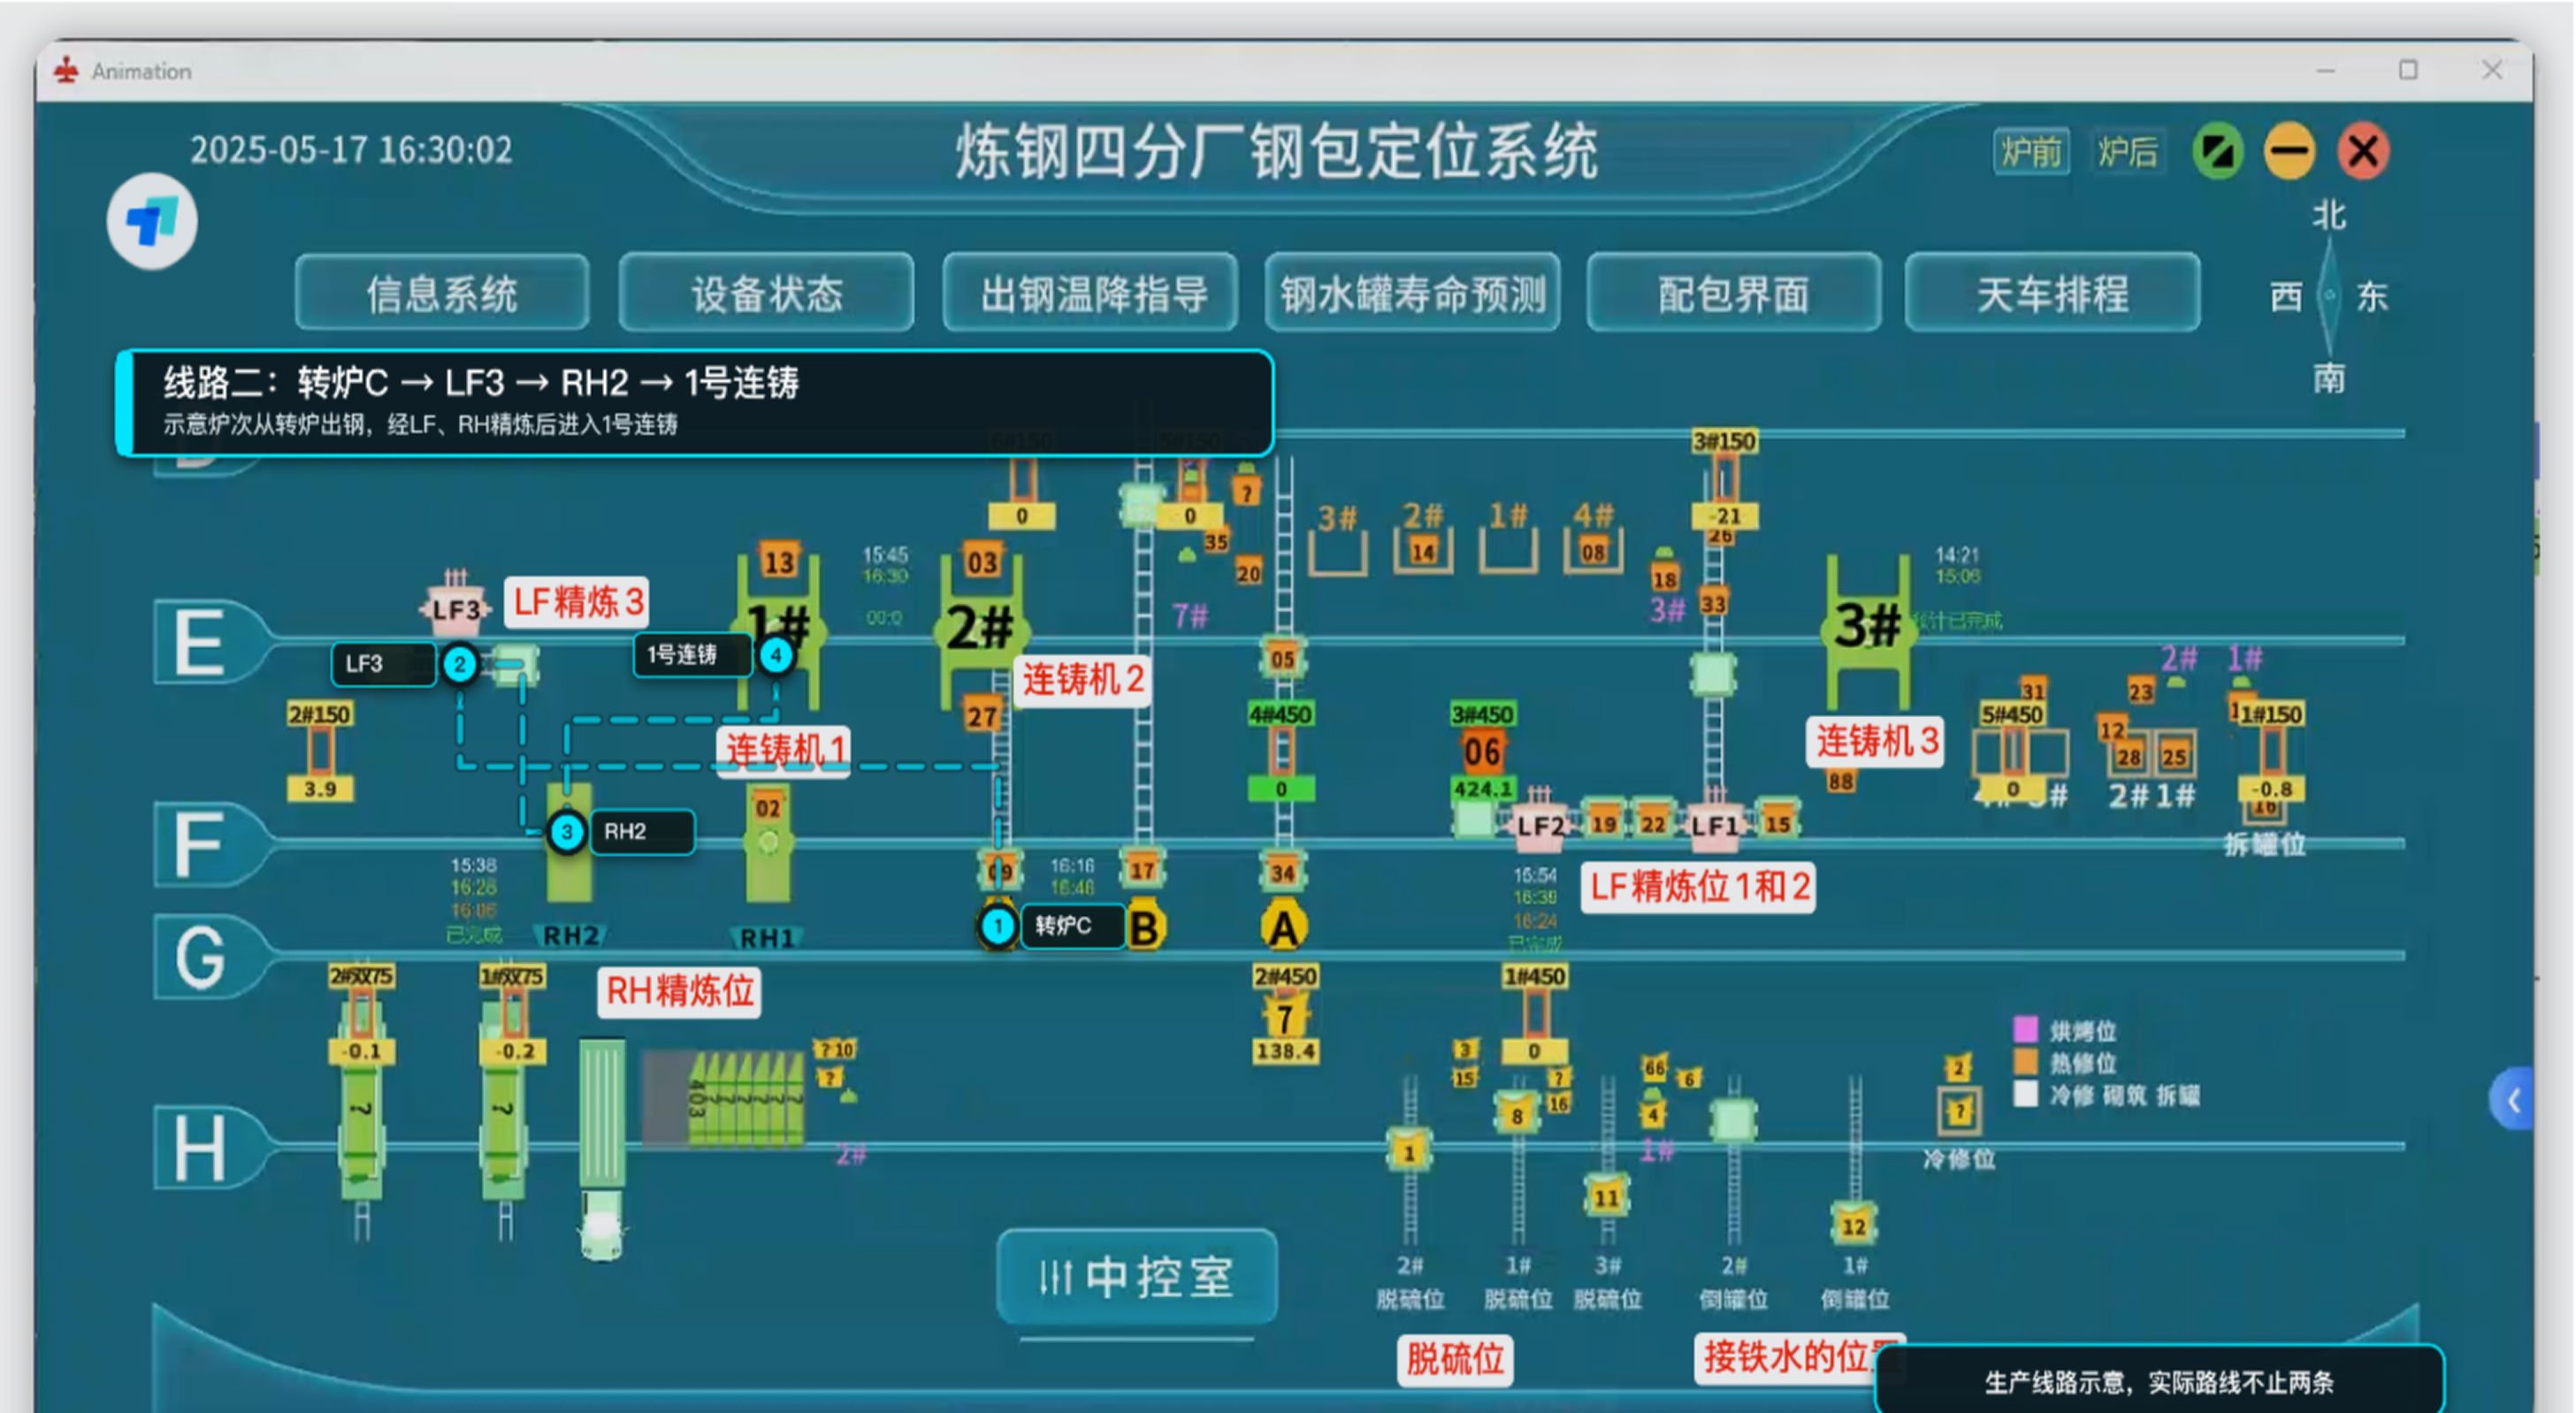
\includegraphics[width=0.95\textwidth]{figures/fig1_plant_layout_raw.png}
  \caption{Plant layout and crane bay schematic showing converters (A/B/C), refining units (LF1--LF3, RH1--RH2), continuous casters (1\#--3\# CCM), transfer cars, and the E--F bay crane ordering.}
  \label{fig:plant_layout}
\end{figure}

\subsection{Problem Decomposition and Unified Architecture}
The problem specifies three progressively richer operational scenarios under a strict lexicographic priority: (i) guarantee safety (zero crane collisions, no overloading, no cast breaks), (ii) minimize ladle waiting time, and (iii) minimize total crane travel time.
\begin{itemize}[leftmargin=1.5em,itemsep=2pt]
  \item \textbf{Scenario 1 (Deterministic Baseline):} Exact planned process times, constant crane speeds, and zero switching delays.
  \item \textbf{Scenario 2 (Stochastic Processing \& Realistic Kinematics):} Random process durations, acceleration/deceleration profiles, discrete speed gears, and spatial slow-down zones.
  \item \textbf{Scenario 3 (Fault-Triggered Rescheduling):} Tapping and ladle-car release uncertainties plus equipment/crane breakdowns while preserving planned casting order.
\end{itemize}

\begin{figure}[htbp]
  \centering
  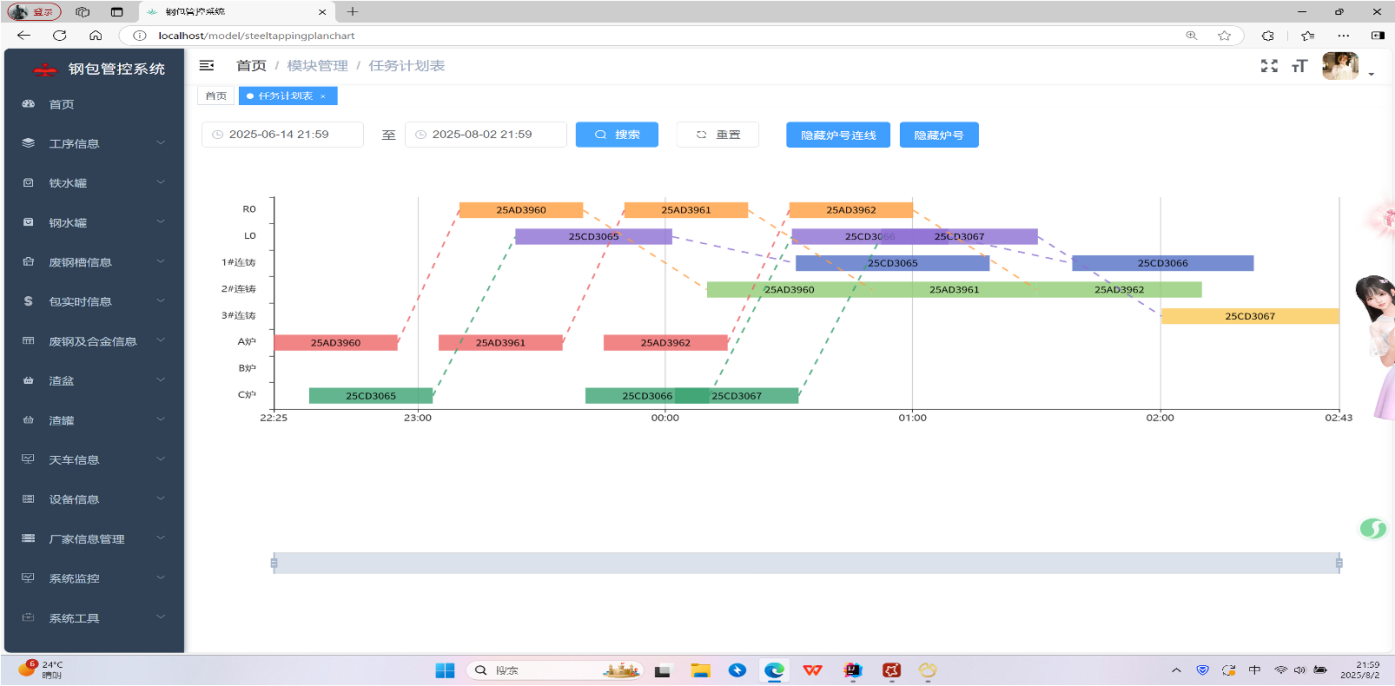
\includegraphics[width=0.90\textwidth]{figures/fig2_mes_gantt_raw.png}
  \caption{Plant MES heat-flow Gantt interface illustrating converter-to-refining-to-caster routing (\texttt{L0}, \texttt{R0}) and inter-stage transfer links.}
  \label{fig:mes_gantt}
\end{figure}

% ============================================================================
% SECTION 2: DATA FORENSICS & EMPIRICAL DIAGNOSIS
% ============================================================================
\section{Multi-Source Data Forensics and Empirical Diagnosis}

\subsection{Non-Destructive Audit of 12 Plant Workbooks}
To establish a reproducible data foundation without silent row deletion, we audited the tapping plan (\texttt{TappingPlan.xls}) and 11 operational Excel logs covering 2026-09-24 23:24 to 2026-10-12 13:04 (6,758 raw rows across 12 SHA-256-verified files). Six \texttt{.xlsx} workbooks contained inaccurate XML dimension headers (\texttt{A1}), requiring full-sheet parsing rather than dimension-reliant read-only mode.

Key empirical findings from \texttt{plan\_audit.json} and \texttt{source\_quality\_summary.csv} include:
\begin{enumerate}[leftmargin=1.5em,itemsep=2pt]
  \item \textbf{Operational Plan Denominator:} Out of 1,321 raw plan rows, 55 carry placeholder flag \texttt{ladle\_alloc\_flag = -2}, leaving \textbf{1,266 unique operational heats} across \textbf{152 continuous casts} (\texttt{cast\_seq\_id}). Every operational row satisfies $(\texttt{tundish\_change} == 1) \Leftrightarrow (\texttt{cast\_order} == 1)$ (205 tundish-change heats, 0 mismatches).
  \item \textbf{Refining Route Mix:} The 1,266 valid heats follow four routes: \texttt{L0} (LF only, 668 heats, 52.8\%), \texttt{R0} (RH only, 420 heats, 33.2\%), \texttt{R0L0} (RH$\rightarrow$LF, 108 heats, 8.5\%), and \texttt{L0R0} (LF$\rightarrow$RH, 70 heats, 5.5\%).
  \item \textbf{Composite Identity Requirement:} While heat IDs (\texttt{heat\_id}) are unique in the tapping plan, the summary log (\texttt{ProcessTimeInfo.xlsx}, 1,355 rows) contains \textbf{72 duplicate heat IDs} (144 rows) bound to distinct ladles and shifted timestamps. Linking solely on \texttt{heat\_id} causes join corruption; we enforce composite \texttt{(heat\_id, ladle\_id)} and temporary ladle ID (\texttt{temp\_ladle\_id}) matching with a fallback time/weight window.
  \item \textbf{Preserved Anomaly Flags (2,529 Review Candidates):} Both RH tables exhibit 533 rows where degassing start equals end time (the reported \texttt{RH\_cycle\_time} field must be used instead); \texttt{3\#LF.xlsx} lacks standby lift time and crane ID in 323 rows; converter \texttt{BOF-B.xlsx} lacks steel-ladle temporary IDs in 435 rows; and four timestamp pairs contain negative-interval candidates (113, 115, 143, and 238 rows) flagged for review rather than clamped to zero.
\end{enumerate}

\subsection{Planned vs. Observed Durations and Physical Crane Asymmetry}
Table~\ref{tab:duration_stats} and Fig.~\ref{fig:data_audit} compare nominal plan durations against clean observed process logs. Nominal plans assign a constant 30.0~min converter slot and fixed inter-stage buffers, whereas actual tapping takes a median of only 5.63~min (P10--P90: 4.47--7.23~min). Furthermore, inspection of crane logs reveals a critical physical asymmetry:
\begin{itemize}[leftmargin=1.5em,itemsep=2pt]
  \item \textbf{E--F Bay Physical Ordering:} From Fig.~\ref{fig:plant_layout}, the west-to-east crane sequence is $\text{2\#150} \prec \text{4\#450} \prec \text{3\#450} \prec \text{5\#450} \prec \text{1\#150}$, which differs from numerical ID order.
  \item \textbf{Why 150~t Cranes Are Bypassed on E--F:} Heavy full ladles weigh 395--421.3~t, exceeding 150~t capacity. Even empty ladles lifted from casters carry residual steel/slag weighing 137.0--150.9~t, repeatedly touching the 150~t limit. Consequently, all observed E--F crane lifts in LF, RH, CCM, and C-BOF logs are executed by \texttt{3\#450}, \texttt{4\#450}, and \texttt{5\#450}, while \texttt{1\#150} and \texttt{2\#150} act as outer-end boundary cranes (and 150~t cranes recorded on A/B-BOF belong to the adjacent D--E bay).
\end{itemize}

\begin{table}[htbp]
\centering
\small
\caption{Planned vs. Clean Observed Process Durations Across All Operational Heats (`basic\_duration\_stats.csv`)}
\label{tab:duration_stats}
\begin{tabular}{llrrrrrr}
\toprule
\textbf{Stage / Metric} & \textbf{Route} & \textbf{$n_{\text{clean}}$} & \textbf{Mean (min)} & \textbf{SD (min)} & \textbf{P10 (min)} & \textbf{Median (min)} & \textbf{P90 (min)} \\
\midrule
Plan Converter & ALL & 1,266 & 30.00 & 0.00 & 30.00 & 30.00 & 30.00 \\
Actual Tapping & ALL & 1,065 & 5.74 & 1.42 & 4.47 & 5.63 & 7.23 \\
Actual LF Process & ALL & 751 & 38.49 & 13.19 & 28.72 & 36.92 & 47.68 \\
Actual RH Process & ALL & 516 & 38.64 & 8.01 & 28.46 & 39.00 & 47.41 \\
Plan Casting & ALL & 1,266 & 41.03 & 3.30 & 37.00 & 40.00 & 46.00 \\
Actual Casting & ALL & 1,117 & 41.45 & 5.00 & 36.23 & 40.65 & 47.89 \\
\bottomrule
\end{tabular}
\end{table}

\begin{figure}[htbp]
  \centering
  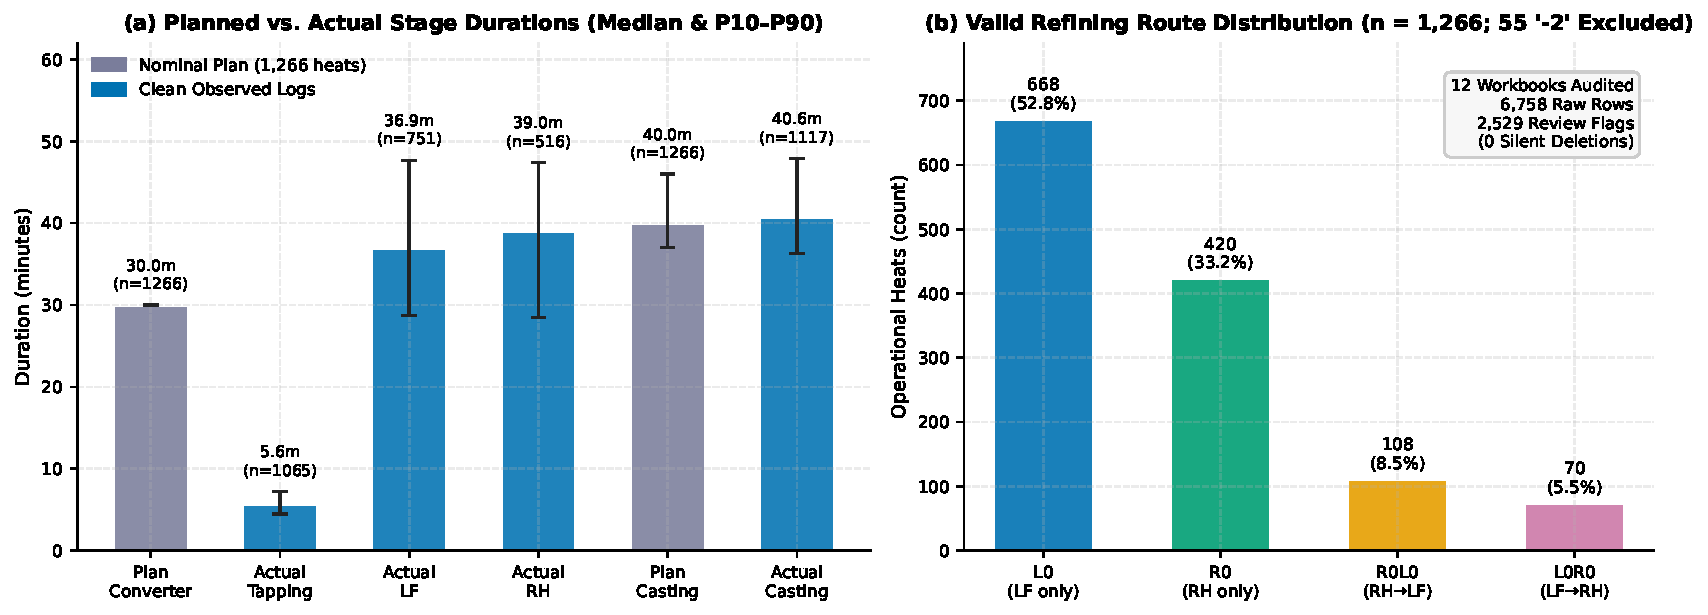
\includegraphics[width=0.96\textwidth]{figures/fig3_data_audit_durations.pdf}
  \caption{(a) Nominal plan vs. clean observed process durations across 1,266 operational heats (median with P10--P90 bars); (b) refining route breakdown and non-destructive source audit totals.}
  \label{fig:data_audit}
\end{figure}

% ============================================================================
% SECTION 3: ASSUMPTIONS, NOMENCLATURE & UNIFIED FORMULATION
% ============================================================================
\section{Assumptions, Nomenclature, and Unified Formulation}

\subsection{Key Modeling Assumptions}
\begin{enumerate}[leftmargin=1.5em,itemsep=2pt]
  \item \textbf{Sufficient Ladle Fleet:} Consistent with the problem statement (26 circulating ladles), ladle shortages do not force artificial heat cancellations; the objective focuses on crane responsiveness and continuity rather than fleet-size minimization.
  \item \textbf{Single-Track Non-Crossing Physics:} All five E--F cranes share one 1D coordinate rail $x \in [0, L]$ in fixed physical order $k \in \{1,\dots,5\}$ ($\text{2\#150}, \text{4\#450}, \text{3\#450}, \text{5\#450}, \text{1\#150}$) and cannot overtake.
  \item \textbf{Load-Dependent Crane Eligibility:} A task $j$ with total lifted mass $w_j$ (steel + ladle + residue) may only be assigned to cranes in $K_j = \{k \in K : w_j \le W_k^{\max}\}$, where $W_k^{\max} \in \{150, 450\}$~t.
  \item \textbf{Transfer-Car Layout Specification:} Consistent with the problem statement and plant schematic (Fig.~\ref{fig:plant_layout}), we model three empty-ladle transfer-car tracks (\texttt{CART1}--\texttt{CART3}, unit capacity 1 ladle) positioned along the east E--F bay, and evaluate sensitivity to transfer-car count and westward relocation in Section~7.
  \item \textbf{Dual-Capacity Refining & Blocking:} Each LF/RH unit separates its receiving/standby berth from its active processing berth; however, a finished ladle remains occupying the station until lifted by a crane.
\end{enumerate}

\subsection{Nomenclature and Four-Class Task Decomposition}
Let $H$ denote operational heats, $O_h$ the ordered process stages of heat $h$, $M$ the stations, and $K$ the five E--F cranes ordered west-to-east. Every E--F crane job $j \in J$ has origin $o_j$, destination $d_j$, earliest ready time $r_j$, due time $b_j$, lifted weight $w_j$, and eligible crane set $K_j$. Following plant logistics, $J$ comprises four coupled classes:
\begin{enumerate}[leftmargin=1.5em,itemsep=2pt]
  \item \textbf{Forward Heavy Transfers ($J^{\text{heavy}}$):} 2 legs for single-refining routes (`L0`, `R0`) and 3 legs for dual-refining routes (`L0R0`, `R0L0`).
  \item \textbf{Post-Casting Empty Returns ($J^{\text{ret}}$):} Direct to transfer cars \texttt{1\#--3\#}, or via slag dumping and/or cast-residue recovery (continuous suspension if handled by one crane, or split into two lifts if handed off).
  \item \textbf{Converter-C Empty Supply ($J^{\text{C-in}}$):} Transfer-car to C-BOF ladle-car seating tasks (`C_IN_h`), specific to converter C (A/B-BOF receive empty ladles via the D--E bay).
  \item \textbf{Cast-Residue Recovery ($J^{\text{rec}}$):} Dual-heat tasks linking donor and receiver heats via \texttt{recovery\_id}.
\end{enumerate}

\subsection{Core Spatio-Temporal Constraints}
For each operation $(h,o)$ with start $S_{ho}$, duration $p_{ho}$, and completion $C_{ho} = S_{ho} + p_{ho}$, and each crane task $j \in J$ with pickup $u_j$, dropoff $v_j$, and assignment $x_{jk} \in \{0,1\}$:
\begin{align}
  u_j &\ge r_j, \qquad \sum_{k \in K_j} x_{jk} = 1, \\
  v_j &= u_j + a_j + T_k(o_j, d_j) + c_j \quad \text{if } x_{jk} = 1, \\
  S_{h,o+1} &\ge v_j \quad \forall \text{ preceding transfer } j \text{ of } (h,o+1), \\
  u_j &\ge v_i + T_k^{\text{empty}}(d_i, o_j) \quad \text{if crane } k \text{ executes } i \to j, \\
  q_{k+1}(t) - q_k(t) &\ge D_k \quad \forall t \ge 0,\; k \in \{1,\dots,4\},
\end{align}
where $a_j, c_j$ are hook-on/hook-off times, $q_k(t)$ is crane $k$'s continuous rail position, and $D_k$ is the minimum center-to-center safety clearance. Within each continuous cast, consecutive heats $(h, h')$ enforce tundish continuity $S_{h',\text{cast}} \ge C_{h,\text{cast}}$ with bounded inter-heat gap and thermal age $S_{h,\text{cast}} - C_{h,\text{last-ref}} \le \Delta_{\text{therm}}^{\max}$.

% ============================================================================
% SECTION 4: SCENARIO 1
% ============================================================================
\section{Scenario 1: Deterministic Scheduling and Cast \texttt{6C0754} Replay}

\subsection{Lexicographic Objective and Breakpoint Safety Property}
In Scenario 1, crane cruise speed $v_k$ is constant ($T_k(o,d) = |d-o|/v_k$) and switching times are zero. Let heat waiting be $W_j = u_j - r_j$ and total crane motion time (loaded plus empty/yielding) be $R$. We minimize the lexicographic objective $\text{lex}\min \big(\text{Violations},\; \sum_{j \in J} W_j,\; R\big)$.

\begin{proposition}[Breakpoint Sufficiency for Constant-Speed Non-Crossing]
Let $\mathcal{T}$ be the union of all trajectory breakpoints (empty-move starts, pickups, dropoffs, and yield-move endpoints) across cranes $k \in K$. Under piecewise-linear trajectories $q_k(t)$ with constant segment velocities, $q_{k+1}(t) - q_k(t) \ge D_k$ holds for all $t \in [0, T_{\max}]$ if and only if it holds at every $t \in \mathcal{T}$.
\end{proposition}
\begin{proof}
On any open interval $(t_m, t_{m+1})$ between consecutive breakpoints in $\mathcal{T}$, both $q_k(t)$ and $q_{k+1}(t)$ are affine functions of $t$. Hence their difference $g_k(t) = q_{k+1}(t) - q_k(t)$ is affine and attains its minimum on $[t_m, t_{m+1}]$ at one of the endpoints $t_m$ or $t_{m+1}$.
\end{proof}

This property enables exact continuous-time MILP verification on single-cast instances and fast conflict-driven yielding in rolling-horizon CP-SAT for full-day schedules.

\subsection{Empirical Replay Benchmark on Cast \texttt{6C0754}}
Before optimizing crane assignments, we replayed cast \texttt{6C0754} (heats \texttt{26BD6452}--\texttt{26BD6457}, all route \texttt{R0}, B-BOF $\rightarrow$ 1\#RH $\rightarrow$ 3\#CCM) using the exact observed crane assignments and timestamps (`run\_id: scene1-replay-6C0754`). As shown in Fig.~\ref{fig:replay_6c0754}:
\begin{itemize}[leftmargin=1.5em,itemsep=2pt]
  \item \textbf{Feasibility & Load Imbalance:} CP-SAT confirms 0 same-crane overlaps (`OPTIMAL` feasibility check), with peak ladle load 421.3~t and empty-return loads 137.0--149.9~t. Crane duty is heavily skewed: \texttt{3\#450} logs 116.87~min versus 72.40~min on \texttt{5\#450} and only 14.35~min on \texttt{4\#450}.
  \item \textbf{Tight Cast Gaps & Thermal Escalation:} Inter-heat casting gaps compress to 1.53--2.78~min, while cast-start delay relative to plan drifts from $-0.93$~min (\texttt{26BD6452}) to $+19.00$~min (\texttt{26BD6457}) and thermal age from RH end to cast start rises from 9.98 to 31.72~min.
\end{itemize}

\begin{figure}[htbp]
  \centering
  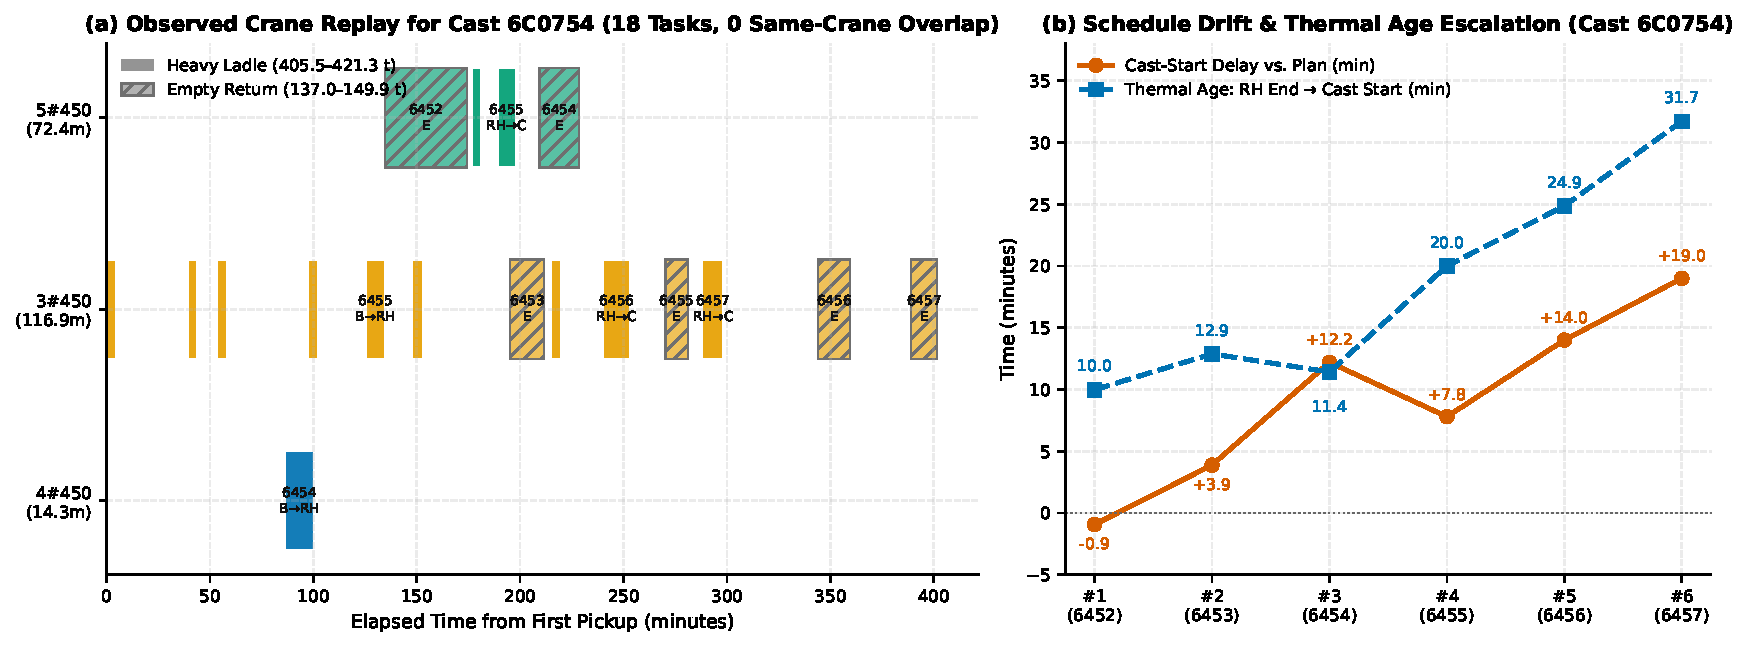
\includegraphics[width=0.96\textwidth]{figures/fig4_replay_6C0754_gantt.pdf}
  \caption{(a) Observed crane assignment Gantt for cast \texttt{6C0754} (18 tasks, 0 same-crane overlaps); (b) progressive schedule drift and thermal age escalation across the 6-heat sequence.}
  \label{fig:replay_6c0754}
\end{figure}

\subsection{Closed-Loop Track Verification and the Need for Proactive Yielding}
Evaluating five candidate policies on the 18-task \texttt{6C0754} closed-loop benchmark under provisional rail geometry (\texttt{scene1\_rail\_params.yml}; Fig.~\ref{fig:closed_loop_6c0754}) uncovers two critical structural insights:
\begin{enumerate}[leftmargin=1.5em,itemsep=2pt]
  \item \textbf{Parallel Dispatch Without Yielding Collides:} Without explicit inter-crane yielding or handoff rules, all four three-crane parallel policies---observed replay (204.12~min wait), FCFS (21.92~min), EDF-Nearest (21.92~min), and CP-SAT with exact empty setup (33.65~min)---violate shared-track separation, producing worst-case crossings of $-1{,}235$ to $-1{,}520$~px against the $+50$~px threshold. Only single-crane \texttt{conservative\_serial} passes ($+60.0$~px clearance), at the cost of inflating task waiting to 109.48~min ($+87.6$~min above FCFS) and lateness to 18.37~min.
  \item \textbf{Empty-Return Calibration Split:} Comparing observed leg durations against heavy-ladle OD regression (\texttt{leg\_calibration.csv}) yields small residuals for \texttt{BOF\_to\_RH} ($+0.89$~min) and \texttt{RH\_to\_CCM} ($+0.87$~min), but a $+12.60$~min residual for \texttt{CCM\_empty\_to\_transfer\_car} (16.02~min observed median vs.\ 3.41~min travel-only prediction) because slag-dumping and residue-handling dwell are embedded in the return leg.
\end{enumerate}

\begin{table}[htbp]
\centering
\small
\caption{Five-Policy Closed-Loop Comparison on Cast \texttt{6C0754} (18 Tasks; Provisional Geometry)}
\label{tab:closed_loop_6c0754}
\begin{tabular}{lrrrrrl}
\toprule
\textbf{Policy} & \textbf{Wait (min)} & \textbf{Lateness (min)} & \textbf{Makespan (min)} & \textbf{Min Gap (px)} & \textbf{Wall (s)} & \textbf{Rail Gate} \\
\midrule
Observed Historical & 204.12 & 14.57 & 401.68 & $-1{,}235.0$ & --- & \textcolor{red!70!black}{Violation} \\
FCFS (No Yield) & 21.92 & 12.09 & 405.12 & $-1{,}520.0$ & --- & \textcolor{red!70!black}{Violation} \\
EDF-Nearest (No Yield) & 21.92 & 12.09 & 405.12 & $-1{,}235.0$ & --- & \textcolor{red!70!black}{Violation} \\
CP-SAT (Exact Setup, No Yield) & 33.65 & 12.08 & 405.12 & $-1{,}520.0$ & 0.044 & \textcolor{red!70!black}{Violation} \\
Conservative Serial (\texttt{5\#450}) & 109.48 & 18.37 & 403.73 & $+60.0$ & 0.024 & \textcolor{green!50!black}{PASS} \\
\bottomrule
\end{tabular}
\end{table}

\begin{figure}[htbp]
  \centering
  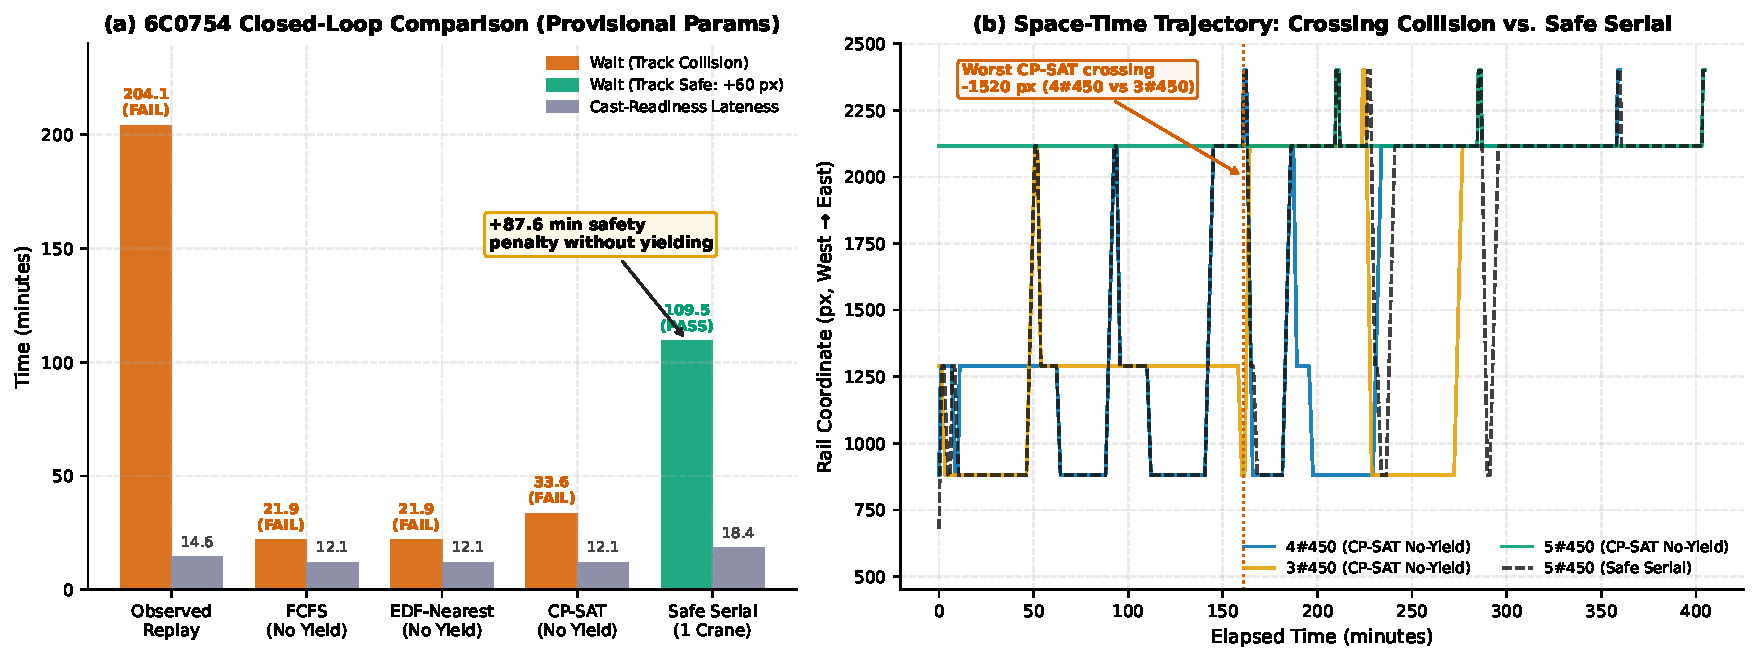
\includegraphics[width=0.96\textwidth]{figures/fig5_closed_loop_6C0754.pdf}
  \caption{(a) Waiting, lateness, and track-safety verdicts across five policies on cast \texttt{6C0754}; (b) space-time trajectories contrasting CP-SAT crossing collisions against the collision-free conservative serial envelope.}
  \label{fig:closed_loop_6c0754}
\end{figure}

\pending{Insert unified ef\_initial\_v1.json proactive-yielding three-crane safe schedule on 6C0754, full-day comparison, and 150~t offload boundary.}

% ============================================================================
% SECTION 5: SCENARIO 2
% ============================================================================
\section{Scenario 2: Multi-Gear Kinematics and Risk-Averse Stochastic Optimization}

\subsection{Piecewise Velocity-Envelope Kinematics}
In Scenario 2, cranes experience finite acceleration/deceleration ($a_k$), discrete speed gears $v_{k,g}$, and spatial slow-down zones $v(x) \le v_{\text{zone}}(x)$ over active tapping or casting turntables. For any move from $x_0$ to $x_1$, the minimum-time feasible speed profile $v(x)$ is computed via a standard forward--backward $v^2(x)$ envelope pass:
\begin{equation}
  v_{\text{fwd}}^2(x + \Delta x) = \min\big(v_{\text{cap}}^2(x+\Delta x),\; v_{\text{fwd}}^2(x) + 2 a_k \Delta x\big), \qquad
  v_{\text{bwd}}^2(x) = \min\big(v_{\text{fwd}}^2(x),\; v_{\text{bwd}}^2(x+\Delta x) + 2 a_k \Delta x\big),
\end{equation}
followed by projection onto the discrete gear set and verification of quadratic relative-displacement extrema ($v_k(t) = v_{k+1}(t)$) inside each segment.

\subsection{Chronological Day-Block Sampling and Rolling SAA-CVaR}
Pure processing durations (tapping, LF, RH, casting) are sampled from empirical distributions stratified by route and equipment using chronological train/validation/test splits without future leakage. At each dispatch epoch, a non-anticipative rolling Sample Average Approximation minimizes expected waiting plus tail tardiness risk:
\begin{equation}
  \min \; \frac{1}{|S|} \sum_{s \in S} \sum_{j \in J} W_{j,s} + \lambda \left( \eta + \frac{1}{(1-\alpha)|S|} \sum_{s \in S} \max(L_s - \eta, 0) \right),
\end{equation}
where $L_s$ is scenario critical cast-readiness tardiness and $(\alpha, \lambda)$ are tuned on the validation split.
\pending{Insert out-of-sample test metrics (mean/P95 wait, cast-break rate, thermal-window violation rate) and phase-plane $(x, v(x))$ figure.}

% ============================================================================
% SECTION 6: SCENARIO 3
% ============================================================================
\section{Scenario 3: Fault-Resilient Rescheduling and Recovery Boundaries}

\subsection{Perturbation Taxonomy and Rail-Partitioning Theorem}
We model both micro-perturbations (tapping delays, argon-station/ladle-car occupancy extending $r_j$) and four macro-faults: BOF, refining (LF/RH), CCM, and crane breakdowns.

\begin{proposition}[Topological Rail Partitioning Under Crane Failure]
If crane $k^*$ fails and remains immobilized at rail coordinate $x_0$, the E--F track is physically partitioned into $[0, x_0 - D_{k^*-1}]$ (accessible only to cranes $k < k^*$) and $[x_0 + D_{k^*}, L]$ (accessible only to cranes $k > k^*$). Any transfer task $j$ with $\min(o_j, d_j) < x_0 < \max(o_j, d_j)$ is physically unreachable without cross-zone equipment substitution or crane towing.
\end{proposition}

\subsection{Event-Triggered Rolling Recovery}
Upon a fault trigger, the rescheduler: (1) updates observable states, (2) freezes completed, in-flight, and short-horizon committed lifts, (3) disables faulted stations/track segments, (4) re-solves with stability penalty $\sum_j |u_j^{\text{new}} - u_j^{\text{old}}|$, and (5) outputs either a verified recovery schedule or an explicit infeasibility diagnosis (affected heats, minimum cast delay, and safe-stop plan).
\pending{Insert 15/30/60~min fault-duration stress-test results, response-time distributions, and recovery Pareto.}

% ============================================================================
% SECTION 7: INDEPENDENT VERIFICATION, ABLATION & SENSITIVITY
% ============================================================================
\section{Independent Verification, Ablation, and Sensitivity Analysis}

Every schedule (`schedule.csv`) and continuous trajectory (`trajectory.csv`) is audited by a standalone black-box verifier checking: (i) exact task coverage, (ii) crane weight limits ($w_j \le W_k^{\max}$), (iii) process precedence and dual-station capacity, (iv) cast continuity and thermal age bounds, and (v) continuous-time rail separation $q_{k+1}(t) - q_k(t) \ge D_k$ including interior quadratic extrema.
\pending{Insert 0-violation audit scorecard, ablation results (proactive yielding, CVaR risk term, stability term), and sensitivity plots.}

% ============================================================================
% SECTION 8: MANAGERIAL INSIGHTS, STRENGTHS & LIMITATIONS
% ============================================================================
\section{Managerial Insights, Strengths, and Limitations}

\subsection{Operational Memo to the Plant Dispatching Center}
\begin{enumerate}[leftmargin=1.5em,itemsep=2pt]
  \item \textbf{Dynamic Zone Control for \texttt{3\#450}:} Because \texttt{3\#450} bridges west (\texttt{4\#450}) and east (\texttt{5\#450}) and carried 116.87~min of duty in cast \texttt{6C0754}, queue-triggered handoff thresholds curb cross-bay interference.
  \item \textbf{Unlocking 150~t Auxiliary Cranes via Slag Control:} Empty ladles off casters reach 149.9--150.9~t; enforcing slag dumping before transfer brings light empty ladles safely below 150~t so \texttt{1\#150}/\texttt{2\#150} can offload \texttt{450~t} cranes.
  \item \textbf{Dual-Key MES Identity Enforcement:} Upgrading MES joins from \texttt{heat\_id} alone to \texttt{(heat\_id, ladle\_id)} + \texttt{temp\_ladle\_id} eliminates the 72 duplicate-heat-ID join ambiguities observed in historical logs.
\end{enumerate}

\subsection{Strengths and Limitations}
\textbf{Strengths:} Non-destructive multi-source data forensics; exact continuous-time breakpoint safety; unified four-class task coverage including C-BOF empty supply and cast-residue recovery; independent black-box verification.\\
\textbf{Limitations:} Metric bay coordinates and kinematic parameters are not explicitly specified in the problem statement and must be calibrated from empirical transit times and sensitivity ranges; long-duration mid-bay crane failures can create physically unreachable transfers requiring manual towing or cast interruption.

% ============================================================================
% REFERENCES
% ============================================================================
\newpage
\bibliographystyle{ieeetr}
\bibliography{refs}

% ============================================================================
% OUTSIDE 25-PAGE LIMIT: AI USE REPORT
% ============================================================================
\newpage
\appendix
\section*{Report on Use of AI}
\addcontentsline{toc}{section}{Report on Use of AI}

In accordance with the competition policy on generative artificial intelligence, this appendix documents all AI tools used during problem analysis, software engineering, and manuscript drafting. All empirical statistics, model constraints, and computational outputs reported in the main text are generated and verified by deterministic Python scripts and solvers in our repository; unexecuted experiments are explicitly marked as pending rather than synthesized.

\begin{table}[htbp]
\centering
\caption{Summary of AI Tool Usage and Verification}
\begin{tabular}{p{3.2cm}p{3.4cm}p{4.5cm}p{4.2cm}}
\toprule
\textbf{Stage} & \textbf{AI Tool / Model} & \textbf{Purpose} & \textbf{Human Verification} \\
\midrule
Problem Structuring \& Literature Discovery & LLM Assistant \& Crossref MCP & Organizing the three-scenario mathematical formulation, identifying data-audit risks, and locating steelmaking scheduling literature. & Cross-checked against the official problem statement, plant layout (Fig.~\ref{fig:plant_layout}), and all 12 raw Excel workbooks. \\
Data Auditing \& ETL Scripting & Coding Assistant & Drafting Python scripts for SHA-256 manifesting, non-destructive anomaly flagging, and duration statistics (\texttt{code/src/}). & Verified via automated \texttt{pytest} unit tests (9 passing checks) and manual trace of heat \texttt{26BD6651} and cast \texttt{6C0754}. \\
Visualization \& LaTeX Drafting & Coding \& Writing Assistant & Generating \texttt{matplotlib} scripts from CSV/JSON outputs and structuring the English LaTeX manuscript. & Every figure and table number traced directly to \texttt{data/audit/} and \texttt{data/runs/} via \texttt{claims\_to\_runs.csv}. \\
\bottomrule
\end{tabular}
\end{table}


\end{document}
